\section{Cell Tracking}
The cell tracking problem is to construct a lineage tree of cells across a time sequence with potentially dividing cells, see Figure~\ref{fig:cell-tracking} for an illustration.
We use a general formulation incorporating mutually exclusive cell candidates originally proposed in~\cite{funke2012efficient}.

\begin{figure}[H]
    \begin{center}
        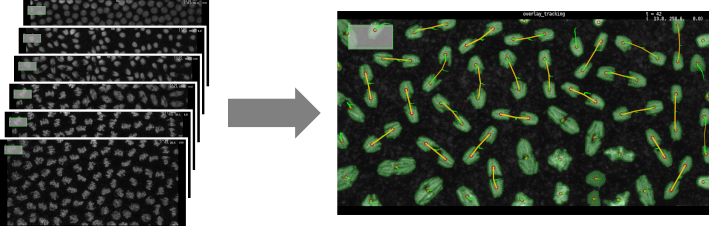
\includegraphics[width=\columnwidth]{images/cell-tracking.png}
        \caption{Cell tracking across timeframes.}
        \label{fig:cell-tracking}
    \end{center}
\end{figure}

\begin{definition}[Cell Tracking]
Let 
$T > 0$ time steps, 
detection candidates $V = V^1 \dot{\cup} \ldots \dot{\cup} V^T$ for each time step,
transition edges $M^t \subset V^t \times V^{t+1}$ and 
division edges $D^t \subset V^t \times \begin{pmatrix}V^{t+1} \\ 2 \end{pmatrix}$ for $t=1,\ldots,T-1$ and 
exclusion sets $\mathcal{E}^t \subset 2^{V^t}$ for $i=1,\ldots,T$
be given.
Define variables
\begin{equation}
\begin{array}{lrl}
    \text{Detection:} &
    x^{det,t} \in \{0,1\}^{V^t} & \forall t \in [T] \\
    \text{Appearance:} &
    x^{app,t} \in \{0,1\}^{V^t} & \forall t \in [T] \\
    \text{Disappearance:} &
    x^{disapp,t} \in \{0,1\}^{V^t} & \forall t \in [T] \\
    \text{Movement:} &
    y^{mov,t} \in \{0,1\}^{M^t} & \forall t \in [T-1] \\
    \text{Division:} &
    y^{div,t} \in \{0,1\}^{D^t} & \forall t \in [T-1] \\
   \end{array}
\end{equation}

The cell tracking problem is
\begin{multline}
\label{eq:cell-tracking-objective}
    \min_{\substack{x^{det}, x^{app}, x^{disapp}\\ y^{mov}, y^{div}}}  
    \la c^{det}, x^{det} \ra 
    + \la c^{app}, x^{app} \ra \\
    + \la c^{disapp}, x^{disapp} \ra 
    + \la c^{mov}, y^{mov} \ra 
    + \la c^{div}, y^{div} \ra 
\end{multline}
such that
    \begin{multline}
        \label{eq:cell-tracking-flow-conservation-incoming}
\forall t \in [T-1], i \in V^t: \\
        \sum_{j \in M^{t}} y^{mov,t}_{ij} + \sum_{j,k: ijk \in D^{t}} x^{div,t}_{ijk} = x^{det,t}_i + x^{disapp,t}_i 
    \end{multline}
    \begin{multline}
        \label{eq:cell-tracking-flow-conservation-outgoing}
\forall t \in [T-1], i \in V^t: \\
    \sum_{i \in M^{t}} y^{mov,t}_{ij} + \sum_{i,k: ijk \in D^{t}} x^{div,t}_{ijk} = x^{det,{t+1}}_j + x^{app,t}_i 
    \end{multline}
    \begin{multline}
        \label{eq:cell-tracking-exclusion-constraint}
        \forall Excl \in \mathcal{E}^t:\\
    \sum_{i \in Excl} x^{det,t}_i \leq 1 
\end{multline}
\end{definition}
The first two constraints in~\eqref{eq:cell-tracking-flow-conservation-incoming} and~\eqref{eq:cell-tracking-flow-conservation-outgoing} are flow conservation constraints stating that whenever a detection is active it must be linked to one detection in the previous timeframe and one or two in the next timeframe.
The third constraint~\eqref{eq:cell-tracking-exclusion-constraint} stipulates that for each exclusion set at most one detection might be active (e.g.\ when multiple cell candidates overlap spatially).

\subsection{File Format}
We use the file format also used in~\cite{haller2020primal}.

\begin{fileformat}
# comment line
# Cell detection hypotheses
H (*$t$*) (*$i$*) (*$c$*)
.
.
.

# Cell appearances, disappearances,
# movement and divisions
APP (*$t$*) (*$i$*) (*$c_{app}$*)
DISAPP (*$t$*) (*$i$*) (*$c_{app}$*)
MOVE (*$id$*) (*$i$*) (*$j$*) (*$c$*)
DIV (*$id$*) (*$i$*) (*$j$*) (*$k$*) (*$c$*)
.
.
.

# Exclusion constraints
CONFSET (*$i_1$*) + ... + (*$i_l$*) <= 1
.
.
.
\end{fileformat}

\begin{description}
    \item[\normalfont Comments] start with \#.
    \item[\normalfont Cell detections] start with `H', next comes the timeframe $t$, then the id $i$ and last the detection cost $c$. The ids must be unique also across timeframes.
    \item[\normalfont Cell appearance/disappearance] start with `APP' (resp.\ `DISAPP'), next comes the timeframe $t$, then the id $i$ and last the appearance/disappearance cost $c$.
    \item[\normalfont Cell movements] start with `MOVE', next come the movement id, then the ids of the two involved cell detections.
    \item[\normalfont Cell divisions] start with `DIV', next come the division id, then the ids of the three involved cell detections.
    \item[\normalfont Exclusion constraints] start with `CONFSET' and uses the ids of the involved cell detections.
\end{description}

We provide LP files for all cell tracking instances as well.

\subsection{Datasets}

\subsubsection[AISTATS 2020 dataset]{AISTATS 2020 dataset\footnote{\url{https://keeper.mpdl.mpg.de/f/da232900c06c46399fd0/?dl=1
}}}
We have taken an extended set of instances used in~\cite{haller2020primal}.
The instances can be grouped as follows.

\paragraph{Drosophila embryo}
One problem instance for tracking nuclei in a developing Drosophila embryo.
The tracking models consists of up tp 252 frames $\sim 320$ detection hypotheses and each and $\sim 160$ true cells.

\paragraph{Flywing}
Tracking membrane-labelled cells in developing Drosophila flywing tissue.
Instances have up to 245 frames with $> 3300$ detection hypotheses per frame.

\paragraph{Cell Tracking Challenge (CTC)}
Publicly available cell tracking instances of sequences from~\cite{ulman2017objective}.
Instances have up to 426 frames and up to 1400 detection hypotheses.

\subsection{Algorithms}
\begin{description}
\item[Primal Dual Solver~\cite{haller2020primal}:] Use dual block coordinate ascent on a Lagrange decomposition and round primal solutions with a series of independent set problems.
\item[Generalized Network Flow~\cite{haubold2016generalized}:] Generalize the successive shortest path minimum cost flow algorithm to efficiently support cell divisions in a network flow model.
\end{description}
